% Provenance (never printed): see sources/outline_sources.md (Year 2: energy geology --- the
% petroleum system quantified, unconventional resources, geothermal systems, uranium deposits,
% geological storage of carbon dioxide).
% Kerogen kinetics and elemental analyses: Fletcher and Pugmire (DOE, OSTI 1176871); kerogen
% types and Easy%Ro: Advanced Chemistry Basins Project (DOE, OSTI 830009); maturity thresholds:
% USGS MF-2008-B; TTI: Waples (1980) and Hammerschmidt et al. (2014); volumetrics and CO2
% storage: DOE/NETL (2008) and IPCC SRCCS (2005) chapter 5; geothermal: USGS OFR 2008-1296 and
% FS 2008-3082; uranium: USGS Bulletin 1693; Oklo: OSTI abstract records. Ledger rows in
% sources/ledger/book4.md; curves from figdata/bachelor-2/maturation.py and co2_density.py,
% numbers from the Book 4 second-writer scratch calculator calc/ch30.py.
% Geology and sourced numbers only: no advocacy, no policy.
\chapter{جيولوجيا الطاقة}\label{ch:b2:energy-geology}

النفط بقايا كائنات مجهرية دُفنت مع الطين وطُهيت ملايين السنين عند
نحو \qty{100}{\celsius}؛ والطاقة الحرارية الأرضية هي دفء الأرض نفسه، مأخوذًا مباشرة.
وتحكم كليهما الحرارةُ والزمن: الأوّل بالمعدّل الذي يجري به تفاعل كيميائي حين
تسخن الصخور المدفونة ببطء، والثاني بكمّية الحرارة التي يختزنها حجم من الصخر وبسرعة نقل الماء
لها إلى بئر. ويقيس هذا الفصل النظام البترولي كمّيًا، ثم ينتقل إلى الموارد التي
ينقصها أحد عناصره، وإلى الحرارة الأرضية وإلى اليورانيوم، ويختم بالعملية المعاكسة:
إعادة ثنائي أكسيد الكربون إلى باطن الأرض.
% ledger: earle:oil-window, earle:organic-preservation

\begin{recall}
\textbf{من مجلّدات المدرسة}: الصخر المصدر، والكيروجين، والنضج، ونافذة النفط، والهجرة،
والصخر الخازن، والصخر الحاجز، والمصيدة، والصخور المغطية، والنظام البترولي؛ والفحم ورتبة الفحم؛ والطاقة الحرارية الأرضية.
\textbf{من مجلّد السنة الأولى}: تدفّق الحرارة والمنحنى الحراري الأرضي؛ والمسامية والنفاذية؛ وضغط سائل
المسام، والإجهاد الفعّال ومعيار كولوم؛ وسجلّ البئر؛ والحوض الرسوبي
والهبوط. \textbf{من كتب الكيمياء}: قانون أرينيوس، وطاقة التنشيط، والتفاعل من الرتبة
الأولى. \textbf{من كتب الفيزياء}: التحلّل الإشعاعي، وثابت التحلّل، وعمر النصف؛ والنقطة
الحرجة للمائع. \textbf{من \cref{ch:b2:basins-compared}}: \omterm{def:b2:basins-compared:curve}{منحنى الهبوط}.
\textbf{من \cref{ch:b2:ore-deposits}}: \omterm{def:b2:ore-deposits:types}{نمط مكامن الخام}، \omterm{def:b2:ore-deposits:grade}{والكتلة الطنّية}.
\end{recall}

\section{النظام البترولي مقيسًا كمّيًا}\label{sec:b2:energy-geology:petroleum}

يحتاج النظام البترولي إلى صخر مصدر غني بالكيروجين، وإلى صخر خازن، وصخر حاجز، ومصيدة، وصخور مغطية كافية
لتسخين الصخر المصدر، ويجب أن تأتي أحداثه بالترتيب الصحيح: فالمصيدة يجب أن تكون
موجودة حين يهاجر النفط. وقياسه كمّيًا يعني الإجابة عن ثلاثة أسئلة: أيّ نوع من الكيروجين
يحوي الصخر المصدر، وإلى أيّ حدّ تحوّل، وكم من الناتج يستقرّ في
المصيدة.
% ledger: magoon00:tps

\begin{definition}[نوع الكيروجين، مخطّط فان كريفلن]\label{def:b2:energy-geology:kerogen}
تنقسم الكيروجينات إلى ثلاثة \emph{أنواع الكيروجين}\index{نوع الكيروجين} بحسب تركيبها العنصري:
النوع~I، السابروبيلي، الأغنى بالهيدروجين، الذي يولّد النفط أساسًا؛ والنوع~III، الدبالي أو الفحمي،
الفقير بالهيدروجين، الذي يولّد الميثان أساسًا؛ والنوع~II، الوسيط، وهو مصدر للنفط
والغاز معًا. و\emph{مخطّط فان كريفلن}\index{مخطّط فان كريفلن} يرسم النسبة الذرية H/C
لكيروجين بدلالة نسبته الذرية O/C؛ وتشغل الأنواع مناطق مختلفة منه، ويُحرّك النضج
الكيروجين نحو قيم منخفضة لكلّ من H/C وO/C.
\end{definition}

لسبعة كيروجينات غير ناضجة معروفة النوع، حُلّلت في دراسة مختبرية واحدة، نسب ذرية H/C قدرها
1.51 و1.61 (النوع~I، ومنها طَفل غرين ريفر النفطي في يوتا، الذي ترسّب في البحيرات وهو غني
ببقايا الطحالب)، ومن 1.22 إلى 1.28 (النوع~II، ومنها طين كيمريدج في بحر الشمال)،
و1.13 (نوع مختلط II/III) و0.99 (النوع~III، فحم كاميو في كولورادو). وكيروجين غرين ريفر،
الذي يبلغ الكربون فيه \qty{77}{\percent} كتليًا، متوسّط صيغته \babelsublr{C$_{100}$H$_{150}$N$_3$O$_8$S}: أي H/C تساوي 1.50
وO/C تساوي 0.08. وعند تسخينه في المختبر بمعدّل \qty{10}{K} في الدقيقة، يترك بقيّة تنخفض نسبتها H/C إلى
1.20 عند \qty{460}{\celsius} وإلى 0.54 عند \qty{525}{\celsius}، بينما تنخفض O/C من 0.08 إلى نحو
0.01: وهو المسار المرسوم على يمين الشكل أدناه.
% ledger: acb04:kerogens, fp14:gr-kerogen, fp14:gr-chars, mf88:thresholds
% values: GR3.9 kerogen H/C 1.486, O/C 0.080; chars 460 C 1.200/0.016, 525 C 0.544/0.011 (figdata maturation.py vk)

\begin{omfigure}
\centering
\begin{minipage}[b]{0.49\linewidth}\centering
\begin{tikzpicture}
\begin{axis}[omrecord, width=0.95\linewidth, height=5.0cm, xmin=0, xmax=0.12, ymin=0, ymax=1.8,
  xlabel={النسبة الذرية \babelsublr{O/C}}, ylabel={النسبة الذرية \babelsublr{H/C}}, xtick={0,0.04,0.08}, scaled x ticks=false,
  xticklabel style={/pgf/number format/fixed}, tick label style={font=\scriptsize},
  label style={font=\small}]
% computed in figdata/bachelor-2/maturation.py part vk; ledger: fp14:gr-kerogen, fp14:gr-chars
\addplot[omThm, line width=0.9pt, mark=*, mark size=1.3pt, -{Stealth[length=4pt]}] table[x=oc, y=hc] {figdata/out/bachelor-2-maturation-vk.dat};
\node[font=\scriptsize, text=omThm, anchor=north east] at (axis cs:0.081,1.45) {كيروجين};
\node[font=\scriptsize, text=omThm, anchor=west] at (axis cs:0.013,0.52) {\qty{525}{\celsius}};
% ledger: acb04:kerogens (H/C of immature kerogens; O/C not reported)
\draw[omThm, line width=1pt] (axis cs:0.104,1.51) -- (axis cs:0.12,1.51);
\draw[omThm, line width=1pt] (axis cs:0.104,1.61) -- (axis cs:0.12,1.61);
\draw[omProp, line width=1pt] (axis cs:0.104,1.22) -- (axis cs:0.12,1.22);
\draw[omProp, line width=1pt] (axis cs:0.104,1.25) -- (axis cs:0.12,1.25);
\draw[omProp, line width=1pt] (axis cs:0.104,1.28) -- (axis cs:0.12,1.28);
\draw[omExo, line width=1pt] (axis cs:0.104,1.13) -- (axis cs:0.12,1.13);
\draw[omDef, line width=1pt] (axis cs:0.104,0.99) -- (axis cs:0.12,0.99);
\node[font=\scriptsize, text=omThm, anchor=east] at (axis cs:0.103,1.58) {I};
\node[font=\scriptsize, text=omProp, anchor=east] at (axis cs:0.103,1.25) {II};
\node[font=\scriptsize, text=omDef, anchor=east] at (axis cs:0.103,0.97) {III};
\end{axis}
\end{tikzpicture}
\end{minipage}\hfill
\begin{minipage}[b]{0.49\linewidth}\centering
\begin{tikzpicture}
\begin{axis}[omrecord, width=0.95\linewidth, height=5.0cm, xmin=60, xmax=220, ymin=0, ymax=1,
  xlabel={درجة الحرارة \babelsublr{(\unit{\celsius})}}, ylabel={نسبة التحوّل},
  tick label style={font=\scriptsize}, label style={font=\small}]
% computed in figdata/bachelor-2/maturation.py part tr; ledger: fp14:gr-daem
\addplot[black!40, densely dotted] coordinates {(60,0.5) (220,0.5)};
\addplot[omDef, line width=1.1pt] table[x=t_c, y=tr1] {figdata/out/bachelor-2-maturation-tr.dat};
\addplot[omThm, line width=1.1pt] table[x=t_c, y=tr10] {figdata/out/bachelor-2-maturation-tr.dat};
\addplot[omDef, line width=0.6pt, densely dashed] table[x=t_c, y=app1] {figdata/out/bachelor-2-maturation-tr.dat};
\addplot[omThm, line width=0.6pt, densely dashed] table[x=t_c, y=app10] {figdata/out/bachelor-2-maturation-tr.dat};
\node[font=\scriptsize, text=omDef, anchor=east] at (axis cs:125,0.80) {\qty{1}{\celsius\per\Myr}};
\node[font=\scriptsize, text=omThm, anchor=west] at (axis cs:160,0.30) {\qty{10}{\celsius\per\Myr}};
\end{axis}
\end{tikzpicture}
\end{minipage}
\par\smallskip{\small يمينًا: \omterm{def:b2:energy-geology:kerogen}{مخطّط فان كريفلن}. والمسار الأحمر هو كيروجين غرين ريفر من النوع~I
وبقاياه بعد تسخينه في المختبر بمعدّل \qty{10}{K} في الدقيقة إلى 400--\qty{525}{\celsius}؛
والعلامات القصيرة على يمين المخطّط تحدّد النسبة H/C لسبعة كيروجينات غير ناضجة من النوع~I (بالأحمر)، وII (بالبرتقالي)،
وII/III (بالرمادي) وIII (بالأزرق)، لم تُذكر نسبتها O/C. البيانات: فليتشر وبوغماير (2014)؛
مشروع أحواض الكيمياء المتقدّمة (2004). يسارًا: نسبة التحوّل لكيروجين غرين ريفر
المسخَّن بمعدّلات ثابتة بدءًا من \qty{10}{\celsius}، بتوزيع طاقات التنشيط الخاصّ به
(المتّصل) وبطاقته المتوسّطة وحدها، وفق \eqref{eq:b2:energy-geology:maturation} (المتقطّع).}
\end{omfigure}

تحوّل الكيروجين إلى بترول مجموعة من التفاعلات من الرتبة الأولى، يخضع كلّ منها لقانون
أرينيوس. وفي حوض هابط ترتفع حرارة الصخر المصدر ببطء وبانتظام
تقريبًا، وهذا ما يجعل النتيجة التالية لبّ نماذج النضج.

\begin{proposition}[تفاعل من الرتبة الأولى بمعدّل تسخين ثابت]\label{prop:b2:energy-geology:maturation}
ليجرِ تفاعل من الرتبة الأولى ثابت معدّله $k = A\,e^{-E/RT}$ في مادّة تُسخَّن بالمعدّل
الثابت $\beta = \mathrm{d}T/\mathrm{d}t$ بدءًا من درجة حرارة $T_0$ يكون عندها $k$ مهملًا.
عندئذ يكون الكسر غير المتحوّل عند درجة الحرارة $T$
\begin{equation}
x(T) = \exp\Bigl[-\frac{A}{\beta}\int_{T_0}^{T} e^{-E/RT'}\,\mathrm{d}T'\Bigr]
\approx \exp\Bigl[-\frac{A R T^2}{\beta E}\,e^{-E/RT}\Bigr] ,
\label{eq:b2:energy-geology:maturation}
\end{equation}
ويصحّ التقريب عندما $E/RT \gg 1$؛ ونسبة التحوّل هي $1 - x$.
\end{proposition}

\begin{proof}
الرتبة الأولى تعني $\mathrm{d}x/\mathrm{d}t = -k x$. ومع $\mathrm{d}t = \mathrm{d}T/\beta$،
يكون $\mathrm{d}\ln x = -(A/\beta)\,e^{-E/RT}\,\mathrm{d}T$، والتكامل من $x = 1$ عند $T_0$ يعطي
الصيغة الأولى. أمّا التكامل، فإنّ $\frac{\mathrm{d}}{\mathrm{d}T}\bigl[\frac{RT^2}{E}e^{-E/RT}\bigr]
= \bigl(1 + \frac{2RT}{E}\bigr)e^{-E/RT}$، فيساوي التكامل $\frac{RT^2}{E}e^{-E/RT}$ إلى حدّ
تصحيح نسبي من رتبة $2RT/E$، إذ لا يسهم الحدّ الأدنى بشيء لأنّ $e^{-E/RT_0} \ll
e^{-E/RT}$.
\end{proof}

وتنتج عن ذلك نتيجتان. يحدث التحوّل على مدى ضيّق من درجات الحرارة، لأنّ
$e^{-E/RT}$ يتغيّر بسرعة كبيرة (التمرين~\ref{exo:b2:energy-geology:11}). والتسخين الأبطأ يُحدث التحوّل
عند درجة حرارة أدنى: فبوضع $x = 1/2$، يرفع معدّل تسخين أسرع بعشر مرّات درجة حرارة
نصف التحوّل بنحو $(RT^2/E)\ln 10$. وحركية كيروجين غرين ريفر، المعايَرة على
الانحلال الحراري في المختبر، هي $A = \qty{9.21e13}{s^{-1}}$ و$E/R = \qty{26800}{K}$ ($E =
\qty{223}{kJ/mol}$)؛ وبهذه الطاقة الوحيدة، يحدث نصف التحوّل عند \qty{136.4}{\celsius} لمعدّل
\qty{1}{\celsius\per\Myr} وعند \qty{150.9}{\celsius} لمعدّل \qty{10}{\celsius\per\Myr}، أي بإزاحة قدرها
\qty{14.5}{\celsius} مقابل $6.26 \times \ln 10 = \qty{14.4}{K}$ متوقَّعة. وعند تسخينه بمعدّل
\qty{10}{K} في الدقيقة، يتحوّل الكيروجين نفسه قرب \qty{450}{\celsius}
(التمرين~\ref{exo:b2:energy-geology:6}): فالزمن يحلّ محلّ درجة الحرارة، ولهذا تُقاس الحركية
بالانحلال الحراري عند نحو 250 إلى \qty{600}{\celsius}، ولهذا يترك استقراؤها عبر اثنتي عشرة
مرتبة عشرية في معدّل التسخين عمقَ نافذة النفط المتوقَّع غير مؤكّد.
% ledger: fp14:gr-daem, acb04:kinetic-spread, codata:R
% values: Thalf 136.403 / 150.873 C; RT2/E 6.2587 K; lab 445.9 C (figdata maturation.py numbers, calc/ch30.py)

والكيروجين الحقيقي يحوي روابط متفاوتة القوّة، فحركيته توزيع من طاقات
التنشيط، يخضع كلّ جزء منه للقضية؛ وفي كيروجين غرين ريفر يكون التوزيع
طبيعيًا، بانحراف معياري $\sigma/R = \qty{481}{K}$. ويوسّع التوزيع
التحوّل، كما يبيّن يسار الشكل: فعند \qty{150}{\celsius} يكون الكيروجين المسخَّن بمعدّل
\qty{1}{\celsius\per\Myr} قد تحوّل بنسبة \qty{93}{\percent}، والمسخَّن بمعدّل أسرع بعشر مرّات
بنسبة \qty{48}{\percent}.
% ledger: fp14:gr-daem
% values: TR 0.927 / 0.484 at 150 C (figdata maturation.py numbers)

\begin{definition}[انعكاسية الفيترينيت، مؤشّر الزمن ودرجة الحرارة]\label{def:b2:energy-geology:maturity}
\emph{انعكاسية الفيترينيت}\index{انعكاسية الفيترينيت}، $R_o$، هي النسبة المئوية للضوء
الساقط التي تعكسها حبيبات مصقولة من الفيترينيت، وهو مكوّن عضوي في الفحم وفي الكيروجين،
وتُقاس تحت المجهر؛ وهي تزداد مع التسخين ازديادًا لا رجعة فيه وتسجّل أعلى نضج حراري بلغه الصخر.
و\emph{مؤشّر الزمن ودرجة الحرارة}\index{مؤشّر الزمن ودرجة الحرارة} (TTI) للوباتين هو المجموع
$\sum_n \Delta t_n\,2^n$ على فترات \qty{10}{\celsius} التي مرّ بها الصخر،
حيث $\Delta t_n$ الزمن بملايين السنين الذي قضاه في الفترة ذات الرقم $n$، مع $n = 0$
للفترة من 100 إلى \qty{110}{\celsius}، و$n = 1$ للفترة من 110 إلى \qty{120}{\celsius}، و$n = -1$ للفترة من 90 إلى
\qty{100}{\celsius}، وهكذا.
\end{definition}

وعلى مقياس الانعكاسية، يبدأ توليد النفط من كيروجينات النوعين~I وII قرب $R_o =
\qty{0.60}{\percent}$؛ وفوق 1.20 إلى \qty{1.30}{\percent} يصبح النفط غير مستقرّ ويتفكّك إلى
ميثان؛ ويبدأ النوع~III بإنتاج الميثان قرب \qty{0.73}{\percent}، ويستمرّ توليد الغاز حتى
نحو \qty{4.8}{\percent}. وتحسب النماذج $R_o$ كما تحسب الكيروجين: فنموذج Easy\%Ro
يعامل الفيترينيت كعشرين تفاعلًا متوازيًا من الرتبة الأولى بثابت $A = \qty{e13}{s^{-1}}$ وطاقات
من 34 إلى \qty{72}{kcal/mol} (من 142 إلى \qty{301}{kJ/mol})، ويحوّل كسرها المتحوّل $F$،
الذي لا يتجاوز 0.85، إلى $R_o = \exp(-1.6 + 3.7F)$، الذي يمتدّ من 0.20 إلى \qty{4.7}{\percent}.
% ledger: mf88:thresholds, acb04:easyro, fp14:gr-chars

وتُحسب الانعكاسية بالطريقة نفسها على طول كلّ أفق في الحوض. ففي الحوض المتخيَّل في
الشكل أدناه، تراكمت الرواسب بمعدّل \qty{100}{m} لكلّ مليون سنة من 100 إلى \qty{70}{\Ma}،
ثم بمعدّل \qty{35}{m} لكلّ مليون سنة، تحت سطح عند \qty{10}{\celsius} وتدرّج ثابت
قدره \qty{30}{\celsius\per\km}. وقد بلغ أقدم أفق فيه $R_o = \qty{0.6}{\percent}$ عند
\qty{67.6}{\Ma}، على عمق \qty{3080}{m} وعند \qty{102}{\celsius}، و\qty{1.3}{\percent} عند
\qty{11.6}{\Ma}، على عمق \qty{5040}{m} وعند \qty{161}{\celsius}؛ وهو الآن على عمق \qty{5450}{m} وعند
\qty{173.5}{\celsius}، بانعكاسية $R_o = \qty{1.54}{\percent}$. ولأنّ المنحنى الحراري الأرضي ثابت، تسير
جبهات الانعكاسية تقريبًا على طول خطوط تساوي الحرارة، وبداية توليد النفط قرب
\qty{100}{\celsius}، ضمن المدى من 60 إلى \qty{120}{\celsius} في مجلّدات المدرسة.
% ledger: acb04:easyro, mf88:thresholds, earle:settings, earle:oil-window
% values: figdata maturation.py numbers (oldest_ro06_*, oldest_ro13_*, ro_oldest_now)

\begin{omfigure}
\centering
\begin{tikzpicture}
\begin{axis}[omrecord, width=0.86\linewidth, height=4.8cm, xmin=0, xmax=100, ymin=0, ymax=5.6,
  x dir=reverse, y dir=reverse, ylabel={العمق \babelsublr{(km)}}, xticklabels={}, name=bh,
  tick label style={font=\scriptsize}, label style={font=\small}]
% computed in figdata/bachelor-2/maturation.py parts burial and fronts (invented basin)
\addplot[black!40, densely dashed] coordinates {(100,1.333) (0,1.333)};
\addplot[black!40, densely dashed] coordinates {(100,3.0) (0,3.0)};
\addplot[black!40, densely dashed] coordinates {(100,4.667) (0,4.667)};
\node[font=\tiny, text=black!60, anchor=south east, fill=white, inner sep=1pt] at (axis cs:1,1.333) {\qty{50}{\celsius}};
\node[font=\tiny, text=black!60, anchor=south east, fill=white, inner sep=1pt] at (axis cs:1,3.0) {\qty{100}{\celsius}};
\node[font=\tiny, text=black!60, anchor=south east, fill=white, inner sep=1pt] at (axis cs:1,4.667) {\qty{150}{\celsius}};
\addplot[black!70, line width=0.5pt, unbounded coords=jump] table[x=t_ma, y expr=\thisrow{d90}/1000] {figdata/out/bachelor-2-maturation-burial.dat};
\addplot[black!70, line width=0.5pt, unbounded coords=jump] table[x=t_ma, y expr=\thisrow{d80}/1000] {figdata/out/bachelor-2-maturation-burial.dat};
\addplot[black!70, line width=0.5pt, unbounded coords=jump] table[x=t_ma, y expr=\thisrow{d70}/1000] {figdata/out/bachelor-2-maturation-burial.dat};
\addplot[black!70, line width=0.5pt, unbounded coords=jump] table[x=t_ma, y expr=\thisrow{d60}/1000] {figdata/out/bachelor-2-maturation-burial.dat};
\addplot[black!70, line width=0.5pt, unbounded coords=jump] table[x=t_ma, y expr=\thisrow{d50}/1000] {figdata/out/bachelor-2-maturation-burial.dat};
\addplot[black!70, line width=0.5pt, unbounded coords=jump] table[x=t_ma, y expr=\thisrow{d40}/1000] {figdata/out/bachelor-2-maturation-burial.dat};
\addplot[black!70, line width=0.5pt, unbounded coords=jump] table[x=t_ma, y expr=\thisrow{d30}/1000] {figdata/out/bachelor-2-maturation-burial.dat};
\addplot[black!70, line width=0.5pt, unbounded coords=jump] table[x=t_ma, y expr=\thisrow{d20}/1000] {figdata/out/bachelor-2-maturation-burial.dat};
\addplot[black!70, line width=0.5pt, unbounded coords=jump] table[x=t_ma, y expr=\thisrow{d10}/1000] {figdata/out/bachelor-2-maturation-burial.dat};
\addplot[black, line width=1.1pt, unbounded coords=jump] table[x=t_ma, y expr=\thisrow{d100}/1000] {figdata/out/bachelor-2-maturation-burial.dat};
\addplot[omDef, line width=1.4pt, unbounded coords=jump] table[x=t_ma, y expr=\thisrow{z06}/1000] {figdata/out/bachelor-2-maturation-fronts.dat};
\addplot[omThm, line width=1.4pt, unbounded coords=jump] table[x=t_ma, y expr=\thisrow{z13}/1000] {figdata/out/bachelor-2-maturation-fronts.dat};
\node[font=\scriptsize, text=omDef, anchor=north, fill=white, inner sep=1pt] at (axis cs:40,3.05) {$R_o = \qty{0.6}{\percent}$};
\node[font=\scriptsize, text=omThm, anchor=north west, fill=white, inner sep=1pt] at (axis cs:9,5.10) {\qty{1.3}{\percent}};
\node[font=\scriptsize, anchor=north east, fill=white, inner sep=1pt] at (axis cs:58,4.75) {الصخر المصدر};
\end{axis}
\begin{axis}[at={(bh.south west)}, anchor=north west, yshift=-0.15cm, width=0.86\linewidth,
  height=2.9cm, xmin=0, xmax=100, ymin=0.4, ymax=6.6, x dir=reverse, y dir=reverse,
  xlabel={الزمن \babelsublr{(\unit{\Ma})}}, ytick={1,2,3,4,5,6},
  yticklabels={الصخر المصدر, الصخر الخازن, الصخر الحاجز, الصخور المغطية, تكوّن المصيدة, التوليد},
  tick label style={font=\tiny}, label style={font=\small}, axis line style={black!60},
  xtick={100,80,60,40,20,0}]
% schematic events chart of the same invented basin
\fill[omLithShale!80!black] (axis cs:100,0.75) rectangle (axis cs:96,1.25);
\fill[omLithSand!70!black] (axis cs:90,1.75) rectangle (axis cs:85,2.25);
\fill[omLithShale!80!black] (axis cs:85,2.75) rectangle (axis cs:80,3.25);
\fill[black!25] (axis cs:80,3.75) rectangle (axis cs:0,4.25);
\fill[omProp!70] (axis cs:75,4.75) rectangle (axis cs:70,5.25);
\fill[omDef!70] (axis cs:67.6,5.75) rectangle (axis cs:11.6,6.25);
\end{axis}
\end{tikzpicture}
\par\smallskip{\small في الأعلى: تاريخ دفن حوض متخيَّل (بالأسود: آفاق ترسّبت كلّ
10 ملايين سنة، والسميك منها هو الصخر المصدر)، وخطوط تساوي الحرارة (متقطّعة)، والأعماق التي يبلغ فيها
نموذج Easy\%Ro القيمة \qty{0.6}{\percent} (بالأزرق) و\qty{1.3}{\percent} (بالأحمر). في الأسفل: مخطّط
أحداثه؛ ويمتدّ التوليد من $R_o = \qty{0.6}{\percent}$ إلى \qty{1.3}{\percent} في الصخر المصدر،
بعد تكوّن المصيدة.}
\end{omfigure}

ومؤشّر TTI أقدم وأخشن. فهو يفترض أنّ النضج يضاعف معدّله مع كلّ
\qty{10}{\celsius}، كما يفعل قانون أرينيوس بطاقة $E \approx \qty{82}{kJ/mol}$ قرب
\qty{100}{\celsius} (التمرين~\ref{exo:b2:energy-geology:5})؛ وعلى مقياسه وضع وابلز بداية
توليد النفط عند مؤشّر 15، وذروته عند 75 ونهايته عند 160.
% ledger: waples80:tti, hamm14:tti-table

\begin{method}[حساب مؤشّر الزمن ودرجة الحرارة]\label{met:b2:energy-geology:tti}
البيانات تاريخ دفن الصخر المصدر والمنحنى الحراري الأرضي، المفترض ثابتًا.
\begin{enumerate}
  \item \textbf{مسار درجة الحرارة.} حوّل العمق إلى درجة حرارة في كلّ لحظة: حرارة السطح
        مضافًا إليها التدرّج مضروبًا في العمق.
  \item \textbf{الأزمنة في الفترات.} أوجد الزمن $\Delta t_n$ المنقضي في كلّ فترة من
        \qty{10}{\celsius}؛ وحيث يكون معدّل التسخين $\beta$ ثابتًا، $\Delta t_n = \qty{10}{\celsius}/\beta$.
  \item \textbf{الجمع.} اجمع الجداءات $\Delta t_n\,2^n$ بترتيب الزمن؛ وتُبلغ بداية توليد النفط وذروته
        ونهايته حين يتجاوز المجموع التراكمي 15 و75 و160.
\end{enumerate}
\end{method}

وتعبّر نماذج الأحواض عن التحوّل بنسبة تحوّل: أي كسر الإمكانية الهيدروكربونية
الأصلية للصخر المصدر الذي تحوّل بالفعل. ففي أحد نماذج حوض في كاليفورنيا،
افتُرض أنّ الطرد من الصخر المصدر يبدأ عند نسبة \qty{10}{\percent}، ويبلغ ذروته عند
\qty{50}{\percent} وينتهي عند \qty{95}{\percent}. والنفط المطرود، الأخفّ من الماء،
يهاجر إلى أعلى نحو صخور خازنة نفوذة، ويُحتجز حيث يُغلق صخر حاجز مصيدةً.
% ledger: peters08b4:tr, magoon00:tps, earle:migration-traps

\begin{proposition}[النفط في المكمن]\label{prop:b2:energy-geology:volumetrics}
لتكن لمصيدة مساحة $A$ ولصخرها الخازن سمك صافٍ $h$ ومسامية $\phi$ وتشبّع مائي
$S_w$، وليكن $B_o$ معامل الحجم التكويني لنفطها، أي نسبة الحجم الذي تشغله كمّية
من النفط في المكمن إلى حجمها عند السطح. إنّ \emph{النفط الأصلي في المكمن بظروف السطح}\index{النفط الأصلي في المكمن بظروف السطح}،
أي حجم النفط مقيسًا عند السطح، هو
\begin{equation}
\mathrm{STOIIP} = \frac{A\,h\,\phi\,(1 - S_w)}{B_o} .
\label{eq:b2:energy-geology:stoiip}
\end{equation}
\end{proposition}

\begin{proof}
الحجم الكلّي للمكمن $Ah$ وحجم مسامه $Ah\phi$؛ ويحوي كسرٌ $1 - S_w$ من
المسام نفطًا، فيشغل النفط $Ah\phi(1 - S_w)$ في المكمن، و$1/B_o$ مرّة من ذلك عند
السطح.
\end{proof}

\begin{definition}[معامل الاستخلاص]\label{def:b2:energy-geology:volumetrics}
\emph{معامل الاستخلاص}\index{معامل الاستخلاص} لمكمن هو كسر النفط (أو الغاز)
الموجود فيه أصلًا الذي يُنتَج على مدى عمره.
\end{definition}

والإنتاج الأوّلي والاستخلاص الثانوي بحقن الماء يستخلصان معًا عادة من 30 إلى \qty{40}{\percent} من النفط في المكمن؛ وحقن ثنائي
أكسيد الكربون يستخلص من 10 إلى \qty{15}{\percent} إضافية. فمصيدة مساحتها \qty{10}{km^2} فيها \qty{30}{m} من
الصخر الخازن الصافي، ومساميته 0.20، وتشبّعه بالنفط 0.70 و$B_o = 1.2$ تحوي \qty{3.5e7}{m^3} من النفط
بظروف السطح، يُنتَج منه من 1.05 إلى \qty{1.4e7}{m^3}.
% ledger: netl08:oilgas

\section{الموارد غير التقليدية}\label{sec:b2:energy-geology:unconventional}

\begin{definition}[المكمن غير التقليدي]\label{def:b2:energy-geology:unconventional}
\emph{المكمن غير التقليدي}\index{المكمن غير التقليدي} صخر نفاذيته من الانخفاض بحيث لا يستطيع
النفط أو الغاز المحتجز في مسامه المجهرية أن يتدفّق إلى بئر بمعدّل اقتصادي
من دون تحفيز اصطناعي؛ ويُنتَج عبر آبار تُحفر أفقيًا على امتداده
وتُكسَّر هيدروليكيًا. ونفط الطَّفل وغاز الطَّفل محتجزان في الصخر المصدر نفسه، والغاز المحكم في
الحجر الرملي والكربونات منخفضة النفاذية.
\end{definition}

فالهدف غير التقليدي إذن صخر مصدر، أو صخر مجاور له، احتفظ بجزء ممّا
ولّده. ونوع الناتج الذي يحويه يتبع درجة نضجه: فالطَّفل في نافذة النفط يحوي نفطًا،
والطَّفل الذي تجاوز $R_o \approx \qty{1.3}{\percent}$ يحوي غازًا. وبدأ الإنتاج الواسع لغاز الطَّفل نحو
عام 2000 في طَفل بارنيت بتكساس، ومعظم نموّ إنتاج الغاز في الولايات المتّحدة منذ
عام 2005 جاء من الحفر الأفقي والتكسير الهيدروليكي في الطَّفل والحجر الرملي والكربونات وغيرها
من التكوينات المحكمة؛ ويُنتَج الغاز أيضًا من طبقات الفحم.
% ledger: eia:shale-gas, eia:gas-coalbed, mf88:thresholds

\section{الطاقة الحرارية الأرضية}\label{sec:b2:energy-geology:geothermal}

\begin{definition}[النظام الحراري الأرضي، الحرارة المختزنة، أصناف الإنثالبي، EGS]\label{def:b2:energy-geology:geothermal}
\emph{النظام الحراري الأرضي}\index{النظام الحراري الأرضي} حجم من القشرة تجتمع فيه الحرارة
والنفاذية والماء بحيث يمكن إنتاج الماء الساخن أو البخار من الآبار.
و\emph{الحرارة المختزنة}\index{الحرارة المختزنة} في مكمن هي الحرارة التي يعطيها حين يبرد
من درجة حرارته إلى درجة حرارة مرجعية. و\emph{المورد عالي الإنثالبي}\index{المورد عالي الإنثالبي}
نظام حراري أرضي تفوق حرارته نحو \qty{150}{\celsius}؛ و\emph{المورد منخفض الإنثالبي}\index{المورد منخفض الإنثالبي}
نظام تقلّ حرارته عن نحو \qty{90}{\celsius}؛ وما بينهما يُسمّى
المورد متوسّطًا. وتصلح الأصناف الثلاثة للاستعمال المباشر للحرارة، لكن عمومًا لا يستطيع توليد الكهرباء إلا الصنفان المتوسّط
والعالي. و\emph{النظام الحراري الأرضي المعزَّز}\index{النظام الحراري الأرضي المعزَّز} (EGS) كتلة من
صخر ساخن منخفض النفاذية الطبيعية تُستحدث فيها النفاذية هندسيًا، بحيث يمكن تدوير الماء
عبرها واستعادة حرارتها.
\end{definition}
% ledger: usgs08g:classes, usgs08g:egs

\begin{proposition}[الحرارة المختزنة والقدرة القابلة للاستعادة]\label{prop:b2:energy-geology:heat}
مكمن حجمه $V$ ومتوسّط حرارته $T_R$ وسعته الحرارية الحجمية $C$ (للصخر وسائل المسام
معًا) يختزن، فوق درجة الحرارة المرجعية $T_0$، الحرارة
\begin{equation}
q_R = C\,V\,(T_R - T_0) .
\label{eq:b2:energy-geology:heat}
\end{equation}
فإذا بلغ كسرٌ $R_g$ منها رؤوس الآبار على مدى زمن إنتاج $\tau$، كانت القدرة الحرارية المتوسّطة
المنتَجة $P = R_g\,q_R/\tau$.
\end{proposition}

\begin{proof}
يُطلق الحجم $\mathrm{d}V$ عند درجة الحرارة $T$ مقدار $C\,\mathrm{d}V\,(T - T_0)$ حين يبرد إلى $T_0$؛
والجمع على المكمن مع $C$ منتظمة يعطي $C\,V\,(T_R - T_0)$ حيث $T_R$ متوسّط
الحرارة. والقدرة هي الحرارة المستعادة مقسومة على الزمن.
\end{proof}

وتستعمل تقييمات الموارد طريقة الحجم هذه بمرجع \qty{15}{\celsius}. ومعامل الاستعادة
$R_g$ هو الجزء غير المؤكّد: فقد أخذت التقييمات المبكّرة 0.25، بين 0 و0.5؛ ويشير الإنتاج من
المكامن المتكسّرة إلى نحو 0.1، بين 0.05 و0.2. ومع $C = \qty{2.5}{MJ.m^{-3}.K^{-1}}$
(تختزن مصفوفات الصخر من 2 إلى \qty{3}{MJ.m^{-3}.K^{-1}})، يختزن مكمن أبعاده $3 \times 4 \times
\qty{1}{km}$ عند \qty{220}{\celsius} مقدار \qty{6.15e18}{J}؛ ومع $R_g = 0.1$ على مدى 30 سنة
يعطي قدرة حرارية متوسّطة قدرها \qty{650}{MW}. وتولّد الحقول التقليدية من 10 إلى
\qty{20}{MW} من الكهرباء لكلّ كيلومتر مربّع من الحقل.
% ledger: usgs08g:volume, delaney86b4:properties, usgs08g:egs
% values: 6.15e18 J; 6.15e17 J; 649.6 MW (calc/ch30.py)

وتحتاج \omterm{def:b2:energy-geology:geothermal}{الأنظمة الحرارية الأرضية} الطبيعية إلى النفاذية بقدر حاجتها إلى الحرارة. ويقع معظم الكبرى منها قرب
حوافّ الصفائح التكتونية، بين البراكين والفومارولات والينابيع الحارّة والفوّارات، ونفاذيتها
عادةً نفاذية كسور فتحها التصدّع النشط: فالمياه الجوفية المسخَّنة في العمق
تصعد عبرها، وتستغلّ الآبار المكمن المتكسّر، كما في المقطع أدناه. أمّا النظام المعزَّز فلا يحتاج إلى مكمن طبيعي:
فآباره، المحفورة إلى نحو \qty{5}{km}، تبلغ صخرًا ساخنًا تُستحدث نفاذيته هندسيًا، وقد
قدّر تقييم أُجري عام 2008 للولايات المتّحدة إمكاناته المؤقّتة بنحو \qty{517800}{MW} من
الكهرباء، مقابل \qty{9057}{MW} من الأنظمة التقليدية المحدَّدة.
% ledger: eia:geo-where, usgs08g:egs, usgs08g:volume

\begin{omfigure}
\centering
\begin{minipage}[b]{0.55\linewidth}\centering
\begin{tikzpicture}[x=0.95cm, y=0.82cm, font=\scriptsize]
% schematic, not to scale
\fill[omLithSand!60] (0,0) -- (7,0) -- (7,-3.6) -- (0,-3.6) -- cycle;
\fill[omProp!35] (1.2,-1.05) .. controls (2.6,-0.85) and (4.4,-0.85) .. (5.8,-1.05)
  -- (5.8,-2.3) .. controls (4.4,-2.5) and (2.6,-2.5) .. (1.2,-2.3) -- cycle;
\fill[omThm!70] (2.6,-3.6) .. controls (2.8,-2.8) and (4.2,-2.8) .. (4.4,-3.6) -- cycle;
\draw[black, line width=0.8pt] (0,0) -- (7,0);
\foreach \x in {1.6,2.4,3.2,4.0,4.8,5.4} {\draw[black!55] (\x,-1.1) -- (\x+0.35,-2.2);}
\draw[omDef, line width=0.9pt, -{Stealth[length=4pt]}] (0.4,-0.1) .. controls (0.5,-2) and (1,-3) .. (2.4,-3.2);
\draw[omDef, line width=0.9pt, -{Stealth[length=4pt]}] (6.6,-0.1) .. controls (6.5,-2) and (6,-3) .. (4.6,-3.2);
\draw[omThm, line width=0.9pt, -{Stealth[length=4pt]}] (3.5,-2.85) -- (3.5,-1.2);
\draw[omThm, line width=0.9pt, -{Stealth[length=4pt]}] (3.5,-1.0) .. controls (3.6,-0.6) .. (5.4,0.02);
\draw[black, line width=1.1pt] (2.9,0.25) -- (2.9,-1.6);
\draw[black, line width=1.1pt] (4.3,0.25) -- (4.3,-1.7);
\fill[black] (2.75,0.25) rectangle (3.05,0.45);
\fill[black] (4.15,0.25) rectangle (4.45,0.45);
\node[anchor=south] at (5.4,0.05) {ينبوع حارّ};
\node[anchor=south] at (2.9,0.45) {بئر};
\node[anchor=south] at (4.3,0.45) {بئر};
\node[text=omDef, anchor=north west] at (0.05,-2.35) {تغذية};
\node[text=omDef, anchor=north west] at (0.05,-2.65) {باردة};
\node[align=center, fill=omProp!20, inner sep=1pt] at (5.1,-1.62) {مكمن\\متكسّر};
\node[text=white] at (3.5,-3.35) {متداخل};
\end{tikzpicture}
\end{minipage}\hfill
\begin{minipage}[b]{0.40\linewidth}\centering
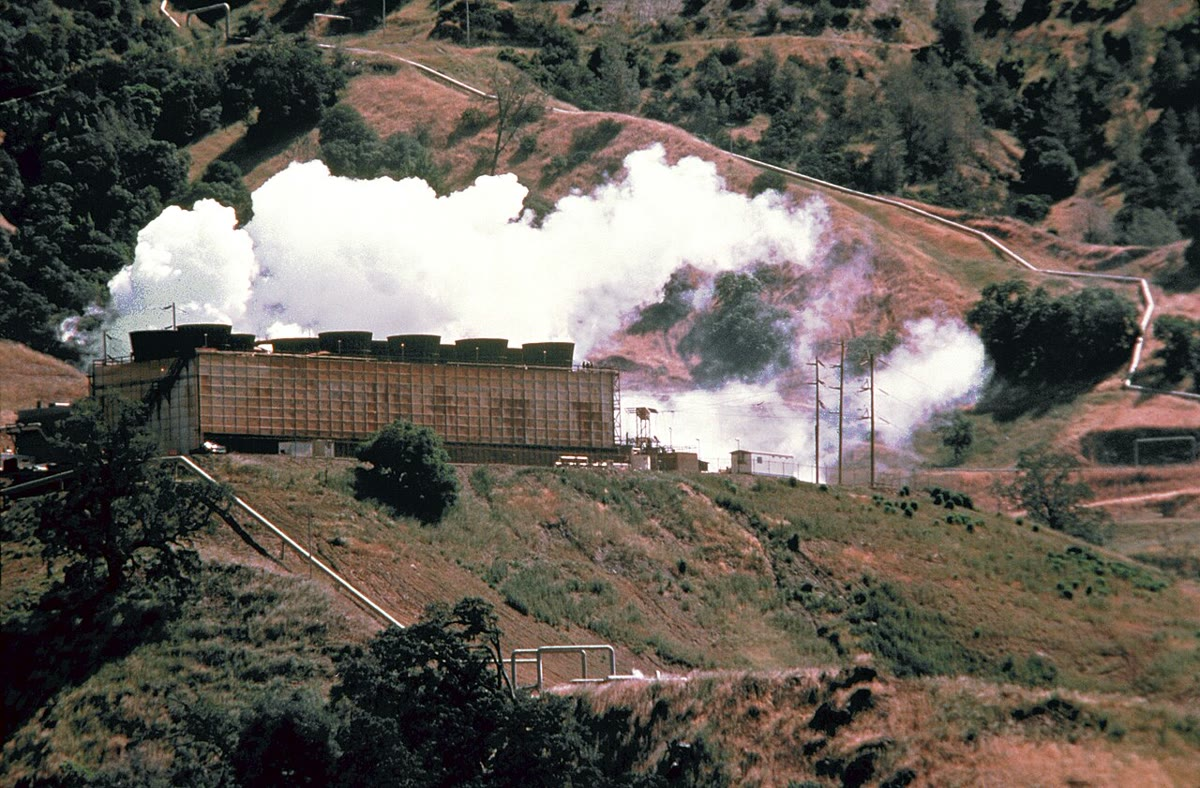
\includegraphics[width=\linewidth]{images/book4/b2-30-geyserville.jpg}
\end{minipage}
\par\smallskip{\small يمينًا: \omterm{def:b2:energy-geology:geothermal}{نظام حراري أرضي} عالي الإنثالبي (رسم تخطيطي، بغير مقياس رسم): الماء
الذي يتغذّى عند الحوافّ (بالأزرق) يُسخَّن فوق متداخل ويصعد عبر مكمن متكسّر
(بالأحمر) إلى ينبوع حارّ؛ وتستغلّ الآبار المكمن. يسارًا: محطّة طاقة حرارية أرضية قرب غيزرفيل،
كاليفورنيا، عام 1982، مع أنابيب البخار على سفح التلّ. الصورة: وزارة الدفاع الأمريكية
(ملك عام).}
\end{omfigure}
% ledger: photo:b2-30-geyserville, usgs08g:egs

\begin{definition}[الزلزالية المستحثّة]\label{def:b2:energy-geology:induced}
\emph{الزلزالية المستحثّة}\index{الزلزالية المستحثّة} نشاط زلزالي تسبّبه عمليات
بشرية تغيّر الإجهاد أو ضغط سائل المسام في القشرة، وأكثرها شيوعًا
حقن الموائع في باطن الأرض.
\end{definition}

والآلية هي معيار كولوم مع ضغط سائل المسام: ينزلق الصدع حين يبلغ إجهاد القصّ
$\mu(\sigma_n - p)$، فرفع $p$ يقرّب صدعًا مُجهَدًا أصلًا من الانهيار
من دون أيّ تغيّر في الحمل التكتوني. ففي ستينيات القرن العشرين، أدّت موائع النفايات المحقونة في
قاعدة ما قبل الكمبري المتكسّرة تحت ترسانة جبال روكي قرب دنفر، على أعماق من 3.7 إلى
\qty{7.0}{km}، إلى إطلاق زلازل؛ وقد اقتصرت على جزء المكمن الذي
ارتفع فيه الضغط بأكثر من \qty{32}{bar} (\qty{3.2}{MPa}). ونُسب الارتفاع الحادّ في زلازل
أوكلاهوما إلى التخلّص من مياه الصرف: فأربع آبار عالية الحجم
قد تفسّر خُمس زلزالية وسط الولايات المتّحدة، مطلقةً
زلازل على بعد أكثر من \qty{30}{km}. وتحفيز مكمن نظام معزَّز يرفع ضغط المسام
بالطريقة نفسها، عن قصد.
% ledger: hb81:denver, keranen:oklahoma, usgs08g:egs

\section{اليورانيوم}\label{sec:b2:energy-geology:uranium}

يوضّح نمطان من مكامن الخام كيف يتركّز اليورانيوم: أحدهما عند عدم توافق قديم، والآخر
في الحجر الرملي.

\begin{definition}[مكامن اليورانيوم المرتبطة بعدم التوافق ومكامن الجبهة الملتفّة]\label{def:b2:energy-geology:uranium}
\emph{مكمن اليورانيوم المرتبط بعدم التوافق}\index{مكمن اليورانيوم المرتبط بعدم التوافق} جسم
من البتشبلند واليورانينيت يملأ الكسور والبريشيا في البيليتات الكربونية المتحوّلة وفي
أرينيتات الكوارتز التي تعلوها، تحت عدم توافق بين صخور \omterm{def:b2:precambrian-earth:eons}{دهر الحياة الطليعية} المبكّر والأوسط أو فوقه أو عبره، في حوض
داخل كراتوني. و\emph{مكمن اليورانيوم ذو الجبهة الملتفّة}\index{مكمن اليورانيوم ذو الجبهة الملتفّة}
جسم هلالي الشكل من معادن اليورانيوم يقطع تطبّق حجر رملي
فلسباري أو طفّي عند الحدّ بين الأرض المؤكسَدة والأرض المختزَلة، حيث
ترسّب اليورانيوم في بيئة مختزَلة محلّيًا، بين البيريت.
\end{definition}

تستضيف مكامنَ عدم التوافق صخورٌ عمرها من 1800 إلى \qty{1200}{\Ma}، هي البيليتات المتحوّلة
تحت عدم التوافق والحجارة الرملية غير المتحوّلة فوقه؛ وصخورها المضيفة مكلورة، والشيست الغرافيتي الذي
يرافق كثيرًا منها موصل كهربائي قويّ، وهدف للمسوح الكهرومغناطيسية. ومن الأمثلة
كي ليك وكلاف ليك ورابيت ليك في ساسكاتشوان وجابيلوكا ورينجر في شمال أستراليا.
أمّا الجبهات الملتفّة فأحدث، ومعظمها من الحقب الثالث: ففي الحجارة الرملية التي يغذّيها رماد بركاني فلسي أو
غرانيت، تقع معادن الحديد المؤكسَدة أعلى الميل من الجبهة والمختزَلة أسفله، كما في أحواض
وايومنغ وساحل الخليج في تكساس.
% ledger: b1693:unconformity, b1693:sandstone

\begin{proposition}[اليورانيوم-235 في الماضي]\label{prop:b2:energy-geology:u235}
لتكن $r_0$ النسبة الذرية الحالية \babelsublr{$^{235}$U/$^{238}$U}، و$\lambda_5$ و$\lambda_8$ ثابتي التحلّل
للنظيرين. فقبل زمن $t$ كانت النسبة
\begin{equation}
r(t) = r_0\,e^{(\lambda_5 - \lambda_8)\,t} ,
\label{eq:b2:energy-geology:u235}
\end{equation}
وكان $^{235}$U يشكّل كسرًا $r/(1 + r)$ من ذرّات اليورانيوم، مع إهمال أثر
$^{234}$U.
\end{proposition}

\begin{proof}
يتحلّل كلّ نظير أسّيًا: $N_5(\text{الآن}) = N_5(t)\,e^{-\lambda_5 t}$ و$N_8(\text{الآن})
= N_8(t)\,e^{-\lambda_8 t}$. وبالقسمة، $r_0 = r(t)\,e^{-(\lambda_5 - \lambda_8)t}$.
\end{proof}

مع $\lambda_5 = \qty{9.8485e-10}{yr^{-1}}$، و$\lambda_8 = \qty{1.55125e-10}{yr^{-1}}$ والوفرتين
الحاليتين \qty{0.7204}{\percent} و\qty{99.2742}{\percent}، يكون $r_0 = 0.0072567$؛ وقبل \qty{2.0}{\Ga}
كانت $r = 0.0381$ وكان اليورانيوم الطبيعي يحوي \qty{3.67}{\percent} من $^{235}$U، أي خمسة أضعاف
حصّته اليوم.
% ledger: amherst:constants, iaea:isotopes
% values: r 0.038144, 3.6743 % (calc/ch30.py)

\begin{history}[مفاعل عمره ملياران من السنين]
في عام 1972، وجد علماء فرنسيون كانوا يقيسون خام اليورانيوم نقصًا صغيرًا لكنّه معتبر في
$^{235}$U، تتبّعوه إلى منجم أوكلو في الغابون. فهناك احتوت جيوب من الصخر ما يصل إلى
\qty{65}{\percent} من اليورانيوم مع نصف الحصّة العادية من $^{235}$U أحيانًا، ونيوديميوم
مستنفَد من نظيره البدئي $^{142}$Nd لكنّه مُثرى بالنظائر من 143 إلى 150 التي ينتجها
الانشطار: فقد جرت تفاعلات متسلسلة في الخام قبل نحو ملياري سنة، عند نحو \qty{300}{bar}
ومن 400 إلى \qty{500}{\celsius}. ويُعرف ستّة عشر مفاعلًا طبيعيًا كهذه في أوكلو وفي
بانغومبي القريبة، وهما المكمنان الوحيدان في العالم اللذان وُجدت فيهما؛ وقد ساعدت المادّة العضوية على
تركيز اليورانيوم، واحتفظ أكسيد اليورانيوم بمعظم الأكتينيدات وبنواتج الانشطار
غير المتطايرة في مكانها منذ ذلك الحين.
\end{history}
% ledger: oklo:curtis, oklo:cowan, oklo:gl96, oklo:nagy

\section{التخزين الجيولوجي لثنائي أكسيد الكربون}\label{sec:b2:energy-geology:ccs}

\begin{definition}[تخزين \ce{CO2} الجيولوجي، آليات الاحتجاز، معامل كفاءة التخزين]\label{def:b2:energy-geology:ccs}
\emph{تخزين \ce{CO2} الجيولوجي}\index{تخزين CO$_2$ الجيولوجي} هو حقن ثنائي أكسيد
الكربون في تكوينات صخرية مسامية عميقة تحت الأرض، أو مكامن نفط وغاز مستنفَدة، أو تكوينات ملحية
عميقة أو طبقات فحم، لاحتجازه مددًا طويلة. و\emph{آليات احتجاز \ce{CO2}}\index{آليات احتجاز CO$_2$}
التي تحتجزه هي الاحتجاز البنيوي (والطبقي) تحت صخر حاجز؛ والاحتجاز المتبقّي، بوصفه طورًا
غير متحرّك تمسكه في المسام القوى الشعرية؛ واحتجاز الذوبان، بانحلاله في ماء التكوين؛
والاحتجاز المعدني، بتفاعله مع المعادن وتحوّله إلى كربونات؛ وفي الفحم والطَّفل، الامتزاز على المادّة العضوية.
و\emph{معامل كفاءة التخزين}\index{معامل كفاءة التخزين} $E$ لتكوين ما هو كسر حجم مسامه الذي يُتوقّع أن يملأه
\ce{CO2} المحقون.
\end{definition}
% ledger: srccs:retention, netl08:saline

ثنائي أكسيد الكربون غاز عند السطح، لكنّ نقطته الحرجة تقع عند \qty{31.0}{\celsius}
و\qty{7.38}{MPa}. وعلى طول منحنى حراري أرضي قدره \qty{25}{\celsius\per\km} بدءًا من \qty{15}{\celsius} تحت
ضغط هيدروستاتيكي، تتجاوز درجة الحرارة القيمة الحرجة عند \qty{641}{m} ويتجاوزها الضغط عند
\qty{742}{m}؛ وتقفز كثافة \ce{CO2} النقيّ من \qty{234}{kg.m^{-3}} عند \qty{700}{m} إلى
\qty{583}{kg.m^{-3}} عند \qty{900}{m}، ثم تستقرّ قرب 670 إلى \qty{700}{kg.m^{-3}} تحت
\qty{1.5}{km}. ويشغل الطنّ الواحد \qty{534}{m^3} عند السطح و\qty{1.6}{m^3} على عمق \qty{1000}{m}،
أي أقلّ بمقدار 330 مرّة؛ ولهذا لا تأخذ تقييمات التخزين في الحسبان إلا التكوينات الأعمق من
\qty{800}{m}.
% ledger: nist:co2-critical, data:b4-co2-density, srccs:density, netl08:saline
% values: z_tc 641.2 m, z_pc 742.2 m; volume ratio 331.9 (figdata co2_density.py numbers)

\begin{omfigure}
\centering
\begin{minipage}[b]{0.49\linewidth}\centering
\begin{tikzpicture}
\begin{axis}[omrecord, width=0.95\linewidth, height=5.2cm, xmin=0, xmax=750, ymin=0, ymax=3,
  y dir=reverse, xlabel={كثافة \ce{CO2} \babelsublr{(\unit{kg.m^{-3}})}}, ylabel={العمق \babelsublr{(km)}},
  tick label style={font=\scriptsize}, label style={font=\small}]
% computed in figdata/bachelor-2/co2_density.py part profile; ledger: data:b4-co2-density
\addplot[black!45, densely dashed] coordinates {(0,0.742) (750,0.742)};
\node[font=\tiny, text=black!60, anchor=south east] at (axis cs:745,0.73) {الضغط الحرج};
\addplot[omDef, line width=1.1pt, mark=*, mark size=0.9pt] table[x=rho, y expr=\thisrow{depth_m}/1000] {figdata/out/bachelor-2-co2_density-profile.dat};
\end{axis}
\end{tikzpicture}
\end{minipage}\hfill
\begin{minipage}[b]{0.49\linewidth}\centering
\begin{tikzpicture}
\begin{axis}[width=0.95\linewidth, height=5.2cm, xmin=0, xmax=4, ymin=0, ymax=100,
  axis x line=bottom, axis y line=left, axis line style={-}, axis on top,
  xlabel={الزمن بعد الحقن (بالسنوات)}, ylabel={حصّة \ce{CO2} المخزَّن},
  xtick={0,1,2,3,4}, xticklabels={1,10,100,1000,$10^4$}, ytick=\empty,
  tick label style={font=\scriptsize}, label style={font=\small}]
% schematic, after IPCC SRCCS (2005) Figure 5.9; ledger: srccs:trapping
% bands from the bottom: mineral, solubility, residual, structural (cumulative tops 0/0/1/5/15,
% 2/8/21/40/60, 10/30/56/80/90, 100)
\fill[omLithLime!60!black] (axis cs:0,0) -- (axis cs:1,0) -- (axis cs:2,1) -- (axis cs:3,5) -- (axis cs:4,15) -- (axis cs:4,0) -- cycle;
\fill[omDef!40] (axis cs:0,0) -- (axis cs:1,0) -- (axis cs:2,1) -- (axis cs:3,5) -- (axis cs:4,15) -- (axis cs:4,60) -- (axis cs:3,40) -- (axis cs:2,21) -- (axis cs:1,8) -- (axis cs:0,2) -- cycle;
\fill[omProp!40] (axis cs:0,2) -- (axis cs:1,8) -- (axis cs:2,21) -- (axis cs:3,40) -- (axis cs:4,60) -- (axis cs:4,90) -- (axis cs:3,80) -- (axis cs:2,56) -- (axis cs:1,30) -- (axis cs:0,10) -- cycle;
\fill[black!15] (axis cs:0,10) -- (axis cs:1,30) -- (axis cs:2,56) -- (axis cs:3,80) -- (axis cs:4,90) -- (axis cs:4,100) -- (axis cs:0,100) -- cycle;
\node[font=\scriptsize] at (axis cs:1.1,72) {البنيوي};
\node[font=\scriptsize] at (axis cs:2.1,38) {المتبقّي};
\node[font=\scriptsize] at (axis cs:3.1,22) {الذوباني};
\node[font=\scriptsize, text=white, anchor=south east] at (axis cs:3.98,0.5) {المعدني};
\end{axis}
\end{tikzpicture}
\end{minipage}
\par\smallskip{\small يمينًا: كثافة \ce{CO2} النقيّ بدلالة العمق على طول منحنى حراري أرضي قدره
\qty{25}{\celsius\per\km} بدءًا من \qty{15}{\celsius}، تحت ضغط هيدروستاتيكي. البيانات: الكتاب الكيميائي على الويب
للمعهد الوطني الأمريكي للمعايير والتقنية (NIST) (معادلة الحالة لسبان وفاغنر)، وفق ظروف التقرير الخاصّ للهيئة الحكومية الدولية
المعنية بتغيّر المناخ عن احتجاز ثنائي أكسيد الكربون وتخزينه (2005). يسارًا: كيف تتقاسم آليات الاحتجاز \ce{CO2} المخزَّن
مع الزمن (رسم تخطيطي، عن التقرير نفسه): يفسح الاحتجاز بالصخر الحاجز المجال للأشكال المتبقّية
والذائبة والمعدنية، وهي أقلّ حركة.}
\end{omfigure}

\begin{proposition}[سعة التخزين في تكوين]\label{prop:b2:energy-geology:capacity}
تكوين مساحته $A$ وسمكه $h$ ومساميته $\phi$، تكون فيه كثافة \ce{CO2} مساوية $\rho$
\omterm{def:b2:energy-geology:ccs}{ومعامل كفاءة التخزين} $E$، يستطيع أن يخزّن الكتلة
\begin{equation}
M = A\,h\,\phi\,\rho\,E .
\label{eq:b2:energy-geology:capacity}
\end{equation}
ولحقل نفط مستنفَد أنتج حجمًا $N_p$ بظروف السطح، فإنّ إحلال الغاز محلّ النفط المنتَج
حجمًا بحجم يعطي $M = \rho\,N_p\,B_o$.
\end{proposition}

\begin{proof}
حجم المسام $Ah\phi$، يملأ \ce{CO2} كسرًا $E$ منه، بكثافة $\rho$. وفي
حقل النفط، كان النفط المنتَج يشغل $N_pB_o$ في المكمن، وهو الحجم الذي يحتلّه \ce{CO2}.
\end{proof}

وفي التكوينات الملحية العميقة، تعطي المحاكاة $E$ بين 1 و\qty{4}{\percent} من حجم المسام
على مدى ثقة من 15 إلى 85 في المئة، بوسيط قرب \qty{2}{\percent}: فمعظم فراغ المسام
لا يُبلغ أبدًا، أو يحتفظ بمائه. وتكوين مساحته \qty{1000}{km^2}، وسمكه \qty{50}{m}،
ومساميته 0.20 على عمق \qty{2000}{m} ($\rho = \qty{686}{kg.m^{-3}}$) يخزّن \qty{137}{Mt} عندما $E =
\qty{2}{\percent}$.
% ledger: netl08:saline, data:b4-co2-density
% values: 1e9*50*0.2*686*0.02 = 1.372e11 kg (calc/ch30.py)

وما إن يُحقن \ce{CO2} حتى يصعد تحت الصخر الحاجز وينتشر. وخلف العمود المهاجر، تمسك القوى
الشعرية تشبّعات متبقّية قد تبلغ من 15 إلى \qty{25}{\percent} من فراغ المسام؛
ويمتصّ الانحلال من 20 إلى \qty{60}{kg} من \ce{CO2} لكلّ متر مكعّب من ماء التكوين، وفي
التكوينات بطيئة الجريان ينحلّ ما يصل إلى \qty{30}{\percent} من \ce{CO2} المحقون خلال عشرات
السنين. ويهيمن احتجاز الذوبان على مدى عشرات إلى مئات السنين، والأشكال الأيونية على مدى مئات إلى
آلاف، والاحتجاز المعدني على مدى آلاف إلى ملايين: فالتفاعلات مع معادن الكربونات تستغرق أيامًا،
ومع السيليكات مئات إلى آلاف السنين. ويصبح التخزين أكثر أمانًا كلّما تقادم، وفي
المواقع المختارة والمدارة جيّدًا حُكم بأنّ احتجاز \qty{99}{\percent} أو أكثر من \ce{CO2} على مدى
1000 سنة مرجح.
% ledger: srccs:trapping, srccs:retention

\begin{dated}{2005}
في سلايبنر، في بحر الشمال على بعد نحو \qty{250}{km} من النرويج، يُحقن \ce{CO2} المفصول عن
الغاز الطبيعي للحقل، وهو نحو \qty{9}{\percent} منه، منذ أكتوبر 1996 في
تكوين أوتسيرا، وهو حجر رملي ملحي غير متماسك يقع من 800 إلى \qty{1000}{m} تحت قاع البحر،
بمعدّل نحو \qty{1}{Mt} في السنة. وبحلول مطلع عام 2005 كان قد خُزّن أكثر من \qty{7}{Mt}، من أصل \qty{20}{Mt}
مخطّط لها على مدى عمر المشروع. وتصوّر المسوح الزلزالية المتكرّرة العمود، الذي كانت بصمته آنذاك
نحو \qty{5}{km^2}، وتُظهر أنّ الصخر الغطائي فوقه يُحكم إغلاقه.
\end{dated}
% ledger: srccs:sleipner

\begin{inthefield}[قراءة بئر أثناء حفرها]
\centering
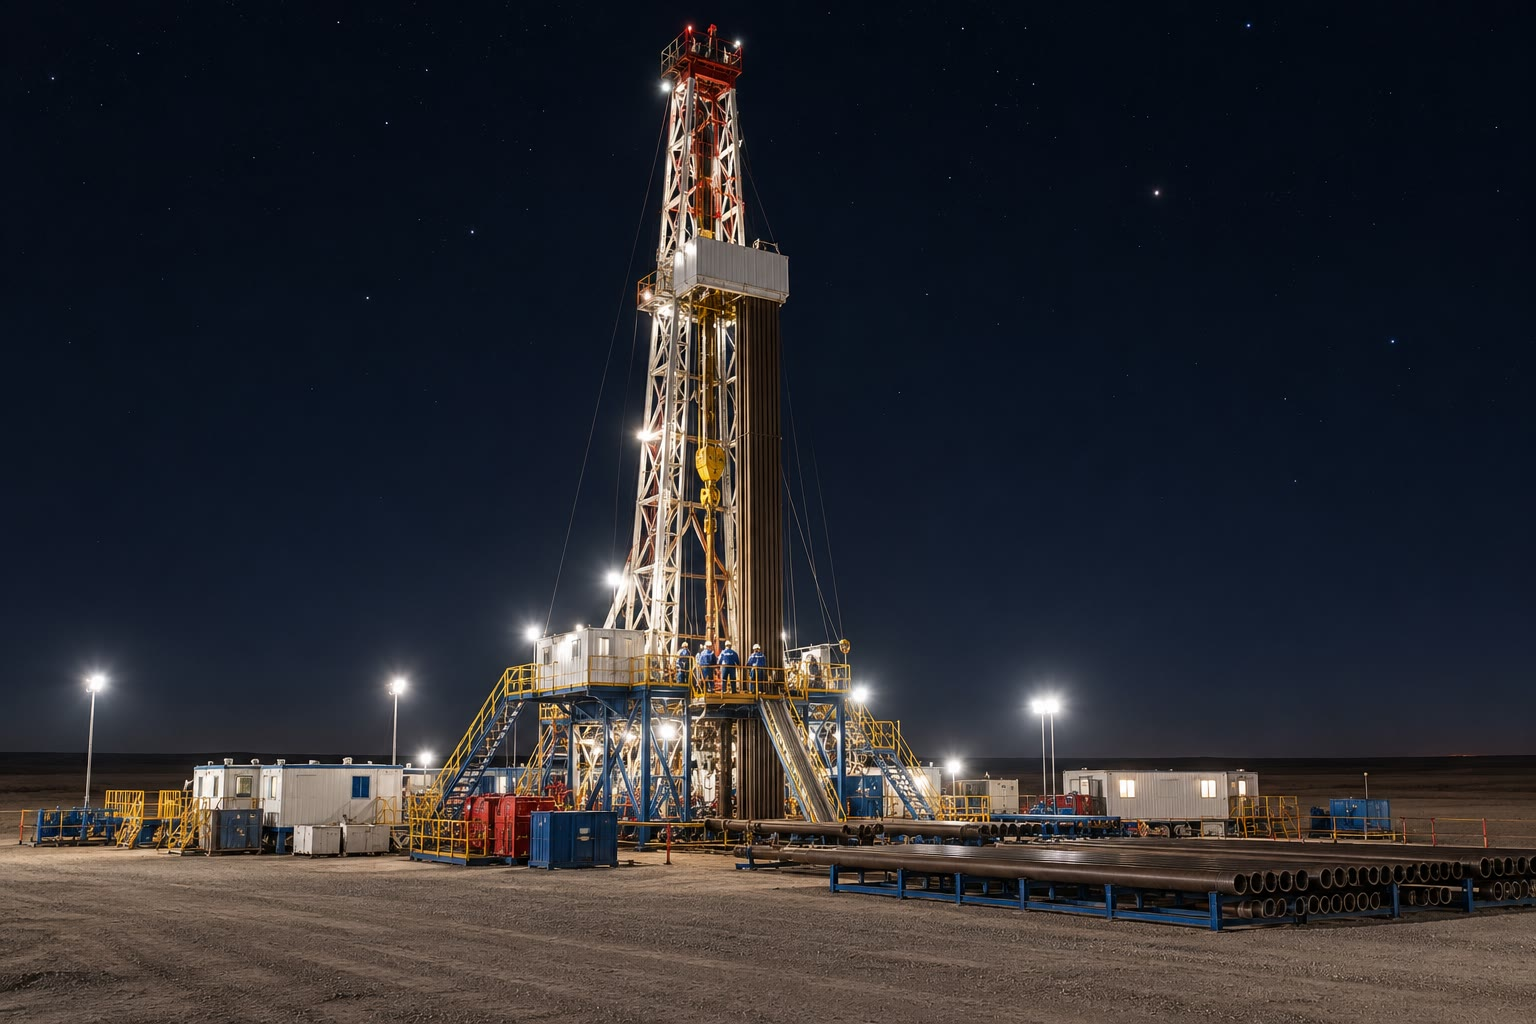
\includegraphics[width=0.56\linewidth]{images/book4/ai/b2-rig-night.jpg}
\par\smallskip{\small جهاز حفر برّي ليلًا (رسم توضيحي مولَّد بالذكاء الاصطناعي).}
\par\medskip\raggedright
حين يكتمل قسم من البئر، يُنزل الجيوفيزيائيون أدوات على كابل ويسجّلون بدلالة
العمق خواصّ الصخور المحيطة بالثقب. فإحداها تسجّل نشاطها الإشعاعي الطبيعي، المنخفض في
الحجر الرملي والأعلى في الطَّفل؛ وأخرى كثافتها الكلّية، التي تُستنتج منها المسامية بالصيغة
(كثافة الحبيبات $-$ الكثافة الكلّية)/(كثافة الحبيبات $-$ كثافة المائع)، مع \qty{2.65}{g/cm^3}
لحبيبات الكوارتز ونحو \qty{1}{g/cm^3} للماء. وعند قراءتها معًا، تعطي سجلّات البئر هذه
سمك الصخر الخازن الصافي والمسامية اللذين يدخلان في الصيغ الحجمية في هذا الفصل.
\end{inthefield}
% ledger: keys:gamma, keys:density-porosity

\section*{التمارين}\label{sec:b2:energy-geology:exercises}

معطيات التمارين، ما لم يُذكر غير ذلك: $R = \qty{8.314}{J.mol^{-1}.K^{-1}}$؛ والمليون
سنة تساوي \qty{3.156e13}{s}؛ وكيروجين غرين ريفر $A = \qty{9.21e13}{s^{-1}}$، و$E/R = \qty{26800}{K}$؛
والكتل الذرية: الكربون 12.011، والهيدروجين 1.008، والأكسجين 15.999؛ وكثافة \ce{CO2} على طول مقطع الشكل:
\qty{1.872}{kg.m^{-3}} عند السطح، و583 عند \qty{900}{m}، و621 عند \qty{1000}{m}، و686 عند
\qty{2000}{m}. قرّب إلى ثلاثة أرقام معنوية.
% ledger: codata:R, fp14:gr-daem, data:b4-co2-density

\begin{exercise}[$\star$]\label{exo:b2:energy-geology:1}
(أ) لأربعة كيروجينات غير ناضجة نسب ذرية H/C قدرها 1.58 و0.95 و1.24 و1.12. حدّد نوع كلّ منها وقل
أيّها يعطي الغاز أساسًا. (ب) تحقّق من النسبتين H/C وO/C للصيغة
\babelsublr{C$_{100}$H$_{150}$N$_3$O$_8$S}. (ج) أوجدهما من التركيب الكتلي: الكربون \qty{77.4}{\percent}، والهيدروجين
\qty{9.8}{\percent}، والأكسجين \qty{8.2}{\percent}.
\end{exercise}

\begin{exercise}[$\star$]\label{exo:b2:energy-geology:2}
(أ) لخمس عيّنات من صخر مصدر من النوع~II قيم $R_o$ = 0.45 و0.68 و1.1 و1.6 و\qty{2.5}{\percent}.
صِف حالة كلّ منها بالنسبة إلى النفط والغاز. (ب) هل يولّد كيروجين من النوع~III عند $R_o =
\qty{0.68}{\percent}$ الميثان؟ (ج) أيّ كسر متحوّل $F$ في نموذج Easy\%Ro يقابل
$R_o = 0.6$ و\qty{1.3}{\percent}؟
\end{exercise}

\begin{exercise}[$\star$]\label{exo:b2:energy-geology:3}
مصيدة مساحتها \qty{6}{km^2}؛ لصخرها الخازن سمك صافٍ \qty{25}{m}، ومسامية 0.18 وتشبّع
مائي 0.30، و$B_o = 1.25$. (أ) أوجد حجم النفط في المكمن والنفط الأصلي بظروف السطح (STOIIP). (ب) أوجد
الحجم المنتَج لمعاملي استخلاص 0.30 و0.40.
\end{exercise}

\begin{exercise}[$\star$]\label{exo:b2:energy-geology:4}
طبقة حاملة للماء من الحجر الرملي سمكها \qty{200}{m} تحت \qty{10}{km^2} عند \qty{75}{\celsius}. (أ) أوجد
\omterm{def:b2:energy-geology:geothermal}{حرارتها المختزنة} فوق \qty{15}{\celsius}، مع $C = \qty{2.5}{MJ.m^{-3}.K^{-1}}$. (ب) إلى أيّ
صنف إنثالبي تنتمي؟ (ج) أوجد القدرة الحرارية المتوسّطة على مدى 30 سنة عندما $R_g = 0.25$.
\end{exercise}

\begin{exercise}[$\star\star$]\label{exo:b2:energy-geology:5}
(أ) أوجد طاقة التنشيط التي يتضاعف عندها معدّل أرينيوس بين 100
و\qty{110}{\celsius}. (ب) بأيّ عامل يزداد معدّل تفاعل غرين ريفر على الفترة
نفسها؟ (ج) أيّ القاعدتين تعطي وزنًا أكبر للزمن الذي قضاه الصخر في درجة حرارة منخفضة،
وماذا يعني ذلك لمؤشّر TTI محسوب لصخر مصدر من النوع~I؟
\end{exercise}

\begin{exercise}[$\star\star$]\label{exo:b2:energy-geology:6}
(أ) بيّن انطلاقًا من \eqref{eq:b2:energy-geology:maturation} أنّ درجة حرارة نصف التحوّل تحقّق
$T = (E/R)\big/\ln\bigl[A T^2/(\beta\,(E/R)\ln 2)\bigr]$، وحلّها بالتكرار لكيروجين غرين
ريفر المسخَّن بمعدّل \qty{1}{\celsius\per\Myr} وبمعدّل \qty{10}{K} في الدقيقة. (ب) قارن
الفرق بالتقدير $(RT^2/E)\ln(\beta_2/\beta_1)$ مأخوذًا عند درجة الحرارة الأدنى، واشرح
سبب التباين.
\end{exercise}

\begin{exercise}[$\star\star$]\label{exo:b2:energy-geology:7}
باستعمال \eqref{eq:b2:energy-geology:u235} ومعطيات النصّ: (أ) أوجد حصّة $^{235}$U في
اليورانيوم الطبيعي قبل \qty{2.0}{\Ga} وقبل \qty{1.8}{\Ga}؛ (ب) متى كانت \qty{3.00}{\percent}؟
(ج) يحوي خام أوكلو أحيانًا نصف الحصّة العادية الحالية من $^{235}$U فقط. بإهمال $^{238}$U
المستهلَك، ما كسر $^{235}$U الموجود وقت التفاعلات الذي انشطر؟ ولماذا
لا يغيّر التحلّل اللاحق الجواب؟
\end{exercise}

\begin{exercise}[$\star\star$]\label{exo:b2:energy-geology:8}
(أ) أوجد حجم \qty{1}{Mt} من \ce{CO2} عند السطح، وعلى عمق \qty{1000}{m} وعلى عمق
\qty{2000}{m}. (ب) في سلايبنر كان قد حُقن أكثر من \qty{7}{Mt} بحلول عام 2005، على عمق نحو
\qty{900}{m}، في عمود بصمته \qty{5}{km^2}. باعتبار مسامية 0.35 وتشبّع بغاز \ce{CO2}
قدره 0.30 في العمود، أوجد حجم الصخر الذي يشغله ومتوسّط سمكه.
\end{exercise}

\begin{exercise}[$\star\star$]\label{exo:b2:energy-geology:9}
مكمن عالي الإنثالبي أبعاده $3 \times 2 \times \qty{1.5}{km}$ عند \qty{250}{\celsius}، مع
$C = \qty{2.6}{MJ.m^{-3}.K^{-1}}$. (أ) أوجد \omterm{def:b2:energy-geology:geothermal}{حرارته المختزنة} فوق \qty{15}{\celsius}. (ب) أوجد
القدرة الحرارية المتوسّطة على مدى 30 سنة عندما $R_g = 0.1$ و$0.25$. (ج) يغطّي حقله \qty{6}{km^2}؛
فبمعدّل 10 إلى \qty{20}{MW} من الكهرباء لكلّ كيلومتر مربّع، ما كسر القدرة الحرارية عندما
$R_g = 0.1$ الذي يصبح كهرباء؟
\end{exercise}

\begin{exercise}[$\star\star\star$]\label{exo:b2:energy-geology:10}
صدع على عمق نحو \qty{4}{km} يحمل إجهادًا عموديًا قدره \qty{80}{MPa} وإجهاد قصّ قدره
\qty{22}{MPa}؛ ومعامل احتكاكه 0.6 وضغط المسام هيدروستاتيكي،
\qty{39}{MPa}. (أ) هل الصدع مستقرّ؟ أوجد ارتفاع ضغط المسام الذي يوصله إلى الانهيار، بالميغاباسكال
وبالبار، وقارن بعتبة دنفر. (ب) الأمر نفسه إذا كان إجهاد القصّ
\qty{24}{MPa}. (ج) اشرح لماذا يمكن إطلاق زلازل على بعد كيلومترات من بئر حقن،
وبعد سنوات من بدء الحقن.
\end{exercise}

\begin{exercise}[$\star\star\star$]\label{exo:b2:energy-geology:11}
(أ) انطلاقًا من التقريب في \eqref{eq:b2:energy-geology:maturation}، بيّن أنّه عند معدّل تسخين
ثابت ترتفع نسبة التحوّل من \qty{10}{\percent} إلى \qty{90}{\percent} على فترة
حرارية $\Delta T \approx \bigl[\ln\ln 10 - \ln\ln(10/9)\bigr]\,RT^2/E$. (ب) احسبها
لكيروجين غرين ريفر عند \qty{1}{\celsius\per\Myr}. (ج) قارن بالمنحنى المتّصل في
الشكل وفسّر الفرق.
\end{exercise}

\begin{exercise}[$\star\star\star$]\label{exo:b2:energy-geology:12}
يُراد أن يخزّن سلايبنر \qty{20}{Mt} من \ce{CO2}. (أ) أوجد حجم ماء التكوين اللازم
لإذابته كلّه، عند 20 وعند \qty{60}{kg.m^{-3}}. (ب) أوجد حجمه طورًا حرًّا على عمق
\qty{1000}{m}. (ج) مع $E = \qty{2}{\percent}$، أوجد حجم المسام اللازم في التكوين،
ومساحة تكوين سمكه \qty{50}{m} ومساميته 0.30.
\end{exercise}
% ledger: srccs:trapping, srccs:sleipner, hb81:denver

\begin{problem}[{مسألة نهاية الأسبوع --- حوض واحد واستعمالان}]\label{pb:b2:energy-geology:1}
في حوض متخيَّل، ترسّب صخر مصدر من النوع~I عند \qty{120}{\Ma} على السطح.
ثم تراكمت الرواسب بمعدّل \qty{60}{m} لكلّ مليون سنة حتى \qty{70}{\Ma}، وبمعدّل \qty{30}{m}
لكلّ مليون سنة منذ ذلك الحين. والسطح عند \qty{15}{\celsius} والمنحنى الحراري الأرضي ثابت عند
\qty{25}{\celsius\per\km}. وللكيروجين حركية غرين ريفر الواردة في النصّ (بطاقة وحيدة).
ومطبخه، أي الجزء الناضج من الصخر المصدر، يغطّي \qty{400}{km^2}، وسمكه \qty{50}{m}
وكثافته \qty{2400}{kg.m^{-3}}، ويمكن أن يعطي \qty{30}{kg} من النفط لكلّ طنّ من الصخر عند
التحوّل الكامل؛ وكثافة النفط عند السطح \qty{850}{kg.m^{-3}}. ويملأ النفط مصيدة مساحتها
\qty{12}{km^2} مركز صخرها الخازن على عمق \qty{2000}{m}، وسمكه الصافي \qty{40}{m}،
ومساميته 0.22 وتشبّعه المائي 0.25، مع $B_o = 1.30$. استعمل معطيات التمارين؛ وقرّب إلى
ثلاثة أرقام معنوية.

\noindent\textbf{الجزء الأول --- الدفن \omterm{def:b2:energy-geology:maturity}{ومؤشّر الزمن ودرجة الحرارة}.}
\begin{enumerate}
  \item أوجد عمق الصخر المصدر ودرجة حرارته عند \qty{70}{\Ma} واليوم.
  \item أوجد معدّل تسخينه في كلّ مرحلة.
  \item أوجد الزمن الذي قضاه في كلّ فترة من \qty{10}{\celsius}، من \qty{15}{\celsius} إلى
        درجة حرارته الحالية.
  \item احسب مؤشّره TTI اليوم (طريقة النصّ).
  \item متى، وعند أيّ درجة حرارة وأيّ عمق، تجاوز مؤشّرًا قدره 15؟
  \item الأمر نفسه للقيمتين 75 و160.
  \item هل لا يزال الصخر المصدر، وفق المؤشّر TTI، يولّد النفط؟
\end{enumerate}

\noindent\textbf{الجزء الثاني --- التحوّل بحسب الحركية.}
\begin{enumerate}[resume]
  \item أوجد ثابت المعدّل عند \qty{90}{\celsius} وبيّن أنّ ما تحوّل من الكيروجين قبل \qty{70}{\Ma}
        لا يمكن أن يتجاوز \qty{0.2}{\percent}.
  \item باستعمال \eqref{eq:b2:energy-geology:maturation} مع معدّل تسخين المرحلة الثانية،
        أوجد الكسر غير المتحوّل ونسبة التحوّل اليوم.
  \item أوجد درجة حرارة نصف التحوّل عند معدّل التسخين هذا (التمرين~\ref{exo:b2:energy-geology:6}).
  \item متى بُلغت؟
  \item قارن بزمن ذروة التوليد الذي يعطيه المؤشّر TTI، وفسّر الفرق.
  \item هل كان كيروجين من النوع~II بطاقة تنشيط متوسّطة أدنى سيتحوّل في وقت أبكر أم في وقت لاحق؟
\end{enumerate}

\noindent\textbf{الجزء الثالث --- النفط المولَّد، والموجود في المكمن، والقابل للاستخلاص.}
\begin{enumerate}[resume]
  \item باعتبار نسبة تحوّل قدرها 0.92، أوجد كتلة النفط المولَّد في المطبخ.
  \item أوجد حجمه عند السطح.
  \item أوجد \omterm{prop:b2:energy-geology:volumetrics}{النفط الأصلي في المكمن بظروف السطح} (STOIIP) للمصيدة.
  \item ما كسر النفط المولَّد الذي تحويه المصيدة؟ احتفظ بالقيمة \qty{1.56e9}{m^3} للسؤال (15).
  \item أوجد النفط المنتَج لمعامل استخلاص قدره 0.35.
  \item لماذا يكون \omterm{def:b2:energy-geology:volumetrics}{معامل الاستخلاص} أقلّ بكثير من الواحد، وماذا يغيّر حقن \ce{CO2}؟
\end{enumerate}

\noindent\textbf{الجزء الرابع --- الحقل المستنفَد مخزنًا لغاز \ce{CO2}.}
\begin{enumerate}[resume]
  \item أوجد درجة حرارة المكمن وضغطه الهيدروستاتيكي. هل يكون \ce{CO2} المحقون
        فوق حرج هناك؟ اقرأ كثافته على الشكل.
  \item مع الاحتفاظ بالقيمة $N_p = \qty{2.13e7}{m^3}$، أوجد حجم المكمن الذي حرّره الإنتاج.
  \item عبّر عنه بمعامل كفاءة تخزين لحجم مسام المصيدة، وقارن
        بالتكوينات الملحية.
  \item يغطّي تكوين ملحي تحت الحقل \qty{600}{km^2}، وسمكه \qty{80}{m}،
        ومساميته 0.20، وكثافة \ce{CO2} فيه \qty{691}{kg.m^{-3}}. أوجد سعته عندما $E =
        \qty{2}{\percent}$.
  \item كم سنة من الحقن بمعدّل سلايبنر تملؤه؟
  \item مع $\rho = \qty{686}{kg.m^{-3}}$ والحجم المحرَّر مقرَّبًا إلى \qty{2.77e7}{m^3}، أوجد
        سعة تخزين \ce{CO2} في المكمن المستنفَد، بالميغاطنّ.
\end{enumerate}
\end{problem}
% ledger: fp14:gr-daem, waples80:tti, hamm14:tti-table, netl08:oilgas, netl08:saline, data:b4-co2-density, nist:co2-critical, srccs:sleipner
